\documentclass[uplatex,dvipdfmx,11pt]{jsarticle}
\usepackage{amsmath,amssymb,amsthm,mathtools}
\usepackage{geometry}
\usepackage{bm}
\usepackage{graphicx}
\usepackage{tikz}
\usetikzlibrary{arrows.meta,positioning}
\usepackage[unicode]{hyperref}
\providecommand{\cInv}{\cos^{-1}}
\providecommand{\E}{\mathrm{E}}
\providecommand{\V}{\mathrm{V}}
\providecommand{\Cov}{\mathrm{Cov}}
\geometry{margin=24mm}

\begin{document}
\begin{center}
{\LARGE\bfseries MORTRA 検証済み解答\par}
\vspace{1mm}
{\small 分野：確率・統計・整数\qquad 問題・厳密解・図・証明経路・講評}
\end{center}
\vspace{1mm}
\hrule
\vspace{5mm}

\section*{問題}
1から$n$までの自然数が書かれたカードが1枚ずつあり,同時に3枚引く.\\
$(1)$ カードの値が三角形の三辺となるような確率$p(n)$を求めよ.また,$\displaystyle \lim_{n\to\infty}p(n)$を求めよ.\\
$(2)$ カードの値が鋭角三角形の三辺となるような確率を$q(n)$とする.$\displaystyle \lim_{n\to\infty}q(n)$を求めよ.

\section*{答え}
\[
p(n)=
\begin{cases}
\dfrac{4r-5}{8r-4}&(n=2r),\\[4pt]
\dfrac{4r^2-3r-1}{8r^2-2}&(n=2r+1),
\end{cases}
\quad(n\ge3),
\qquad
\lim_{n\to\infty}p(n)=\frac12,
\qquad
\lim_{n\to\infty}q(n)=1-\frac\pi4.
\]

\section*{解答}
\textbf{1.} 三枚の値は相異なるから、小さい順に \(1\le a<b<c\le n\) と一意に並べられる。全事象の個数は \({}_{n}C_3\) である。最大辺は \(c\) なので、三角形にならないための必要十分条件は \(a+b\le c\) である。

\textbf{2.} \(c=2s\) のとき、\(b=2,\ldots,s\) では \(a\) が \(b-1\) 通り、\(b=s+1,\ldots,2s-1\) では \(2s-b\) 通りである。従って個数は \(s(s-1)\) である。\(c=2s+1\) のときも同様に \(s^2\) 個となる。まとめると \[\#\{(a,b):1\le a<b<c,\ a+b\le c\}=\left\lfloor\frac{(c-1)^2}{4}\right\rfloor.\]

\textbf{3.} \(N_{n}\) を非三角形の組数とし、\(m=c-1\) と置く。床関数を偶奇に分けると \[\begin{aligned}N_{2r}&=\sum_{j=1}^{r-1}\{j^2+j(j+1)\}=\frac{r(r-1)(4r+1)}6,\\N_{2r+1}&=\sum_{j=1}^rj^2+\sum_{j=1}^{r-1}j(j+1)=\frac{r(r+1)(4r-1)}6.\end{aligned}\] よって \(1-N_{n}/{}_{n}C_3\) を整理すれば \[p(n)=\begin{cases}\dfrac{4r-5}{8r-4}&(n=2r),\\[3pt]\dfrac{4r^2-3r-1}{8r^2-2}&(n=2r+1)\end{cases}\] を得る。どちらの式も \(r\to\infty\) で \(1/2\) に近づく。

\textbf{4.} 次に鋭角三角形を数える。最大辺が \(c\) なので、その条件は \(a^2+b^2>c^2\) である。\(a/n,b/n,c/n\) を改めて \(a,b,c\) と書くと、整数格子点の比は領域 \[0<a<b<c<1,\qquad a^2+b^2>c^2\] の体積比へ近づく。不等号が等号となる境界は面だけからなり体積が0なので、極限値には影響しない。

\textbf{5.} \(c\) と \(b\) を固定すると、\(a\) の範囲は \(\sqrt{c^2-b^2}<a<b\) である。この区間が存在するのは \(c/\sqrt2<b<c\) のときである。従って鋭角領域の体積 \(V\) は \[\begin{aligned}V&=\int_0^1\int_{c/\sqrt2}^{c}\left(b-\sqrt{c^2-b^2}\right)\,db\,dc\\&=\frac13\int_{1/\sqrt2}^{1}\left(t-\sqrt{1-t^2}\right)\,dt.\end{aligned}\] ここで二つの積分は \[\int_{1/\sqrt2}^{1}t\,dt=\frac14,\qquad \int_{1/\sqrt2}^{1}\sqrt{1-t^2}\,dt=\frac\pi8-\frac14\] だから、\(V=(4-\pi)/24\) となる。

\textbf{6.} 一方、全ての順序付き領域 \(0<a<b<c<1\) の体積は \(1/6\) であり、\({}_{n}C_3/n^3\to1/6\) と一致する。従って \[\lim_{n\to\infty}q(n)=\frac{(4-\pi)/24}{1/6}=1-\frac\pi4.\]

\clearpage

\section*{一手ずつ見る図解}

\subsection*{1. 三枚を小さい順に並べる}

同時に引いた三枚は相異なるため、三枚を a、b、c と名づけて小さい順に一意に並べます。最大の値を c とすれば、残り二つの和が c より大きいことだけを調べればよくなります。

\[
1\le a<b<c\le n,\qquad a+b>c
\]

\begin{center}

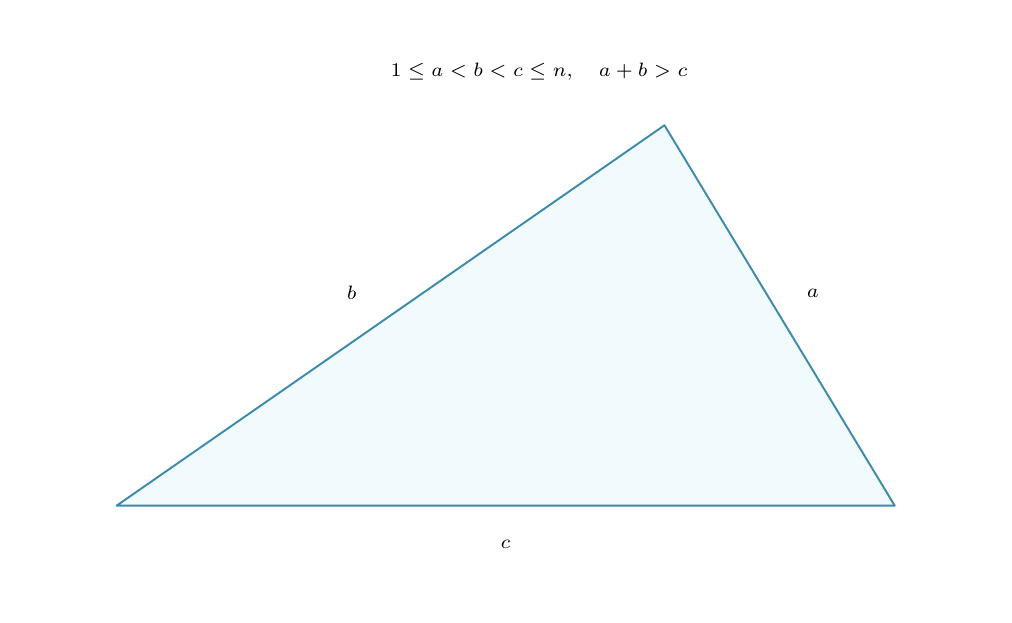
\begin{tikzpicture}[scale=1.411765,line cap=round,line join=round]
\path[use as bounding box] (-0.80000000,-0.80000000) rectangle (7.80000000,4.30000000);
\draw[draw=cyan!65!black,fill=cyan!10,line width=.7pt,fill opacity=.55] (0.00000000,0.00000000) -- (7.00000000,0.00000000) -- (4.92857143,3.42186845) -- cycle;
\node[font=\scriptsize,fill=white,inner sep=1.5pt] at (3.50000000,-0.35000000) {\(c\)};
\node[font=\scriptsize,fill=white,inner sep=1.5pt] at (2.11428571,1.91093422) {\(b\)};
\node[font=\scriptsize,fill=white,inner sep=1.5pt] at (6.26428571,1.91093422) {\(a\)};
\node[font=\scriptsize,fill=white,inner sep=1.5pt] at (3.80000000,3.90000000) {\(1\le a<b<c\le n,\quad a+b>c\)};
\end{tikzpicture}

\end{center}

\subsection*{2. 最大辺ごとに非三角形を数える}

最大の値 c を固定し、残り二つの和が c 以下となる整数の組を図の格子点として数えます。c が偶数でも奇数でも、個数は直後の一つの式にまとまります。

\[
\#\{(a,b):1\le a<b<c,\ a+b\le c\}=\left\lfloor\frac{(c-1)^2}{4}\right\rfloor
\]

\begin{center}

\begin{tikzpicture}[scale=0.782609,line cap=round,line join=round]
\path[use as bounding box] (0.00000000,0.00000000) rectangle (9.20000000,9.20000000);
\draw[->,black!35] (0.00000000,0)--(9.20000000,0);
\draw[->,black!35] (0,0.00000000)--(0,9.20000000);
\draw[draw=black!38,line width=.7pt,densely dashed] (1.00000000,1.00000000) -- (8.30000000,8.30000000);
\draw[draw=magenta!70!black,line width=.7pt] (1.00000000,8.00000000) -- (8.00000000,1.00000000);
\node[font=\scriptsize,fill=white,inner sep=1.5pt] at (8.65000000,0.35000000) {\(b\)};
\node[font=\scriptsize,fill=white,inner sep=1.5pt] at (0.35000000,8.65000000) {\(a\)};
\node[font=\scriptsize,fill=white,inner sep=1.5pt] at (6.70000000,2.65000000) {\(a+b=9\)};
\fill[magenta!70!black] (2.00000000,1.00000000) circle (1.25pt);
\fill[magenta!70!black] (3.00000000,1.00000000) circle (1.25pt);
\fill[magenta!70!black] (4.00000000,1.00000000) circle (1.25pt);
\fill[magenta!70!black] (5.00000000,1.00000000) circle (1.25pt);
\fill[magenta!70!black] (6.00000000,1.00000000) circle (1.25pt);
\fill[magenta!70!black] (7.00000000,1.00000000) circle (1.25pt);
\fill[magenta!70!black] (8.00000000,1.00000000) circle (1.25pt);
\fill[magenta!70!black] (3.00000000,2.00000000) circle (1.25pt);
\fill[magenta!70!black] (4.00000000,2.00000000) circle (1.25pt);
\fill[magenta!70!black] (5.00000000,2.00000000) circle (1.25pt);
\fill[magenta!70!black] (6.00000000,2.00000000) circle (1.25pt);
\fill[magenta!70!black] (7.00000000,2.00000000) circle (1.25pt);
\fill[cyan!65!black] (8.00000000,2.00000000) circle (1.25pt);
\fill[magenta!70!black] (4.00000000,3.00000000) circle (1.25pt);
\fill[magenta!70!black] (5.00000000,3.00000000) circle (1.25pt);
\fill[magenta!70!black] (6.00000000,3.00000000) circle (1.25pt);
\fill[cyan!65!black] (7.00000000,3.00000000) circle (1.25pt);
\fill[cyan!65!black] (8.00000000,3.00000000) circle (1.25pt);
\fill[magenta!70!black] (5.00000000,4.00000000) circle (1.25pt);
\fill[cyan!65!black] (6.00000000,4.00000000) circle (1.25pt);
\fill[cyan!65!black] (7.00000000,4.00000000) circle (1.25pt);
\fill[cyan!65!black] (8.00000000,4.00000000) circle (1.25pt);
\fill[cyan!65!black] (6.00000000,5.00000000) circle (1.25pt);
\fill[cyan!65!black] (7.00000000,5.00000000) circle (1.25pt);
\fill[cyan!65!black] (8.00000000,5.00000000) circle (1.25pt);
\fill[cyan!65!black] (7.00000000,6.00000000) circle (1.25pt);
\fill[cyan!65!black] (8.00000000,6.00000000) circle (1.25pt);
\fill[cyan!65!black] (8.00000000,7.00000000) circle (1.25pt);
\end{tikzpicture}

\end{center}

\subsection*{3. 偶数項と奇数項を別々に足す}

床関数を偶数項と奇数項の二つに分け、非三角形の総数と p(n) を有限式にします。

\[
\left\lfloor\frac{(2j)^2}{4}\right\rfloor=j^2,\qquad \left\lfloor\frac{(2j+1)^2}{4}\right\rfloor=j(j+1)
\]

\begin{center}

\begin{tikzpicture}[scale=1.302083,line cap=round,line join=round]
\path[use as bounding box] (1.20000000,-0.12000000) rectangle (10.80000000,1.28000000);
\draw[->,black!35] (1.20000000,0)--(10.80000000,0);
\node[font=\scriptsize,fill=white,inner sep=1.5pt] at (10.55000000,-0.04000000) {\(m\)};
\node[font=\scriptsize,fill=white,inner sep=1.5pt] at (1.55000000,1.15000000) {\(\lfloor m^2/4\rfloor\)};
\draw[draw=cyan!65!black,line width=.7pt] (2.00000000,0.00000000) -- (2.00000000,0.04000000);
\fill[cyan!65!black] (2.00000000,0.04000000) circle (1.25pt);
\node[font=\scriptsize,fill=white,inner sep=1.5pt] at (2.00000000,0.11000000) {\(1\)};
\draw[draw=magenta!70!black,line width=.7pt] (3.00000000,0.00000000) -- (3.00000000,0.08000000);
\fill[magenta!70!black] (3.00000000,0.08000000) circle (1.25pt);
\node[font=\scriptsize,fill=white,inner sep=1.5pt] at (3.00000000,0.15000000) {\(2\)};
\draw[draw=cyan!65!black,line width=.7pt] (4.00000000,0.00000000) -- (4.00000000,0.16000000);
\fill[cyan!65!black] (4.00000000,0.16000000) circle (1.25pt);
\node[font=\scriptsize,fill=white,inner sep=1.5pt] at (4.00000000,0.23000000) {\(4\)};
\draw[draw=magenta!70!black,line width=.7pt] (5.00000000,0.00000000) -- (5.00000000,0.24000000);
\fill[magenta!70!black] (5.00000000,0.24000000) circle (1.25pt);
\node[font=\scriptsize,fill=white,inner sep=1.5pt] at (5.00000000,0.31000000) {\(6\)};
\draw[draw=cyan!65!black,line width=.7pt] (6.00000000,0.00000000) -- (6.00000000,0.36000000);
\fill[cyan!65!black] (6.00000000,0.36000000) circle (1.25pt);
\node[font=\scriptsize,fill=white,inner sep=1.5pt] at (6.00000000,0.43000000) {\(9\)};
\draw[draw=magenta!70!black,line width=.7pt] (7.00000000,0.00000000) -- (7.00000000,0.48000000);
\fill[magenta!70!black] (7.00000000,0.48000000) circle (1.25pt);
\node[font=\scriptsize,fill=white,inner sep=1.5pt] at (7.00000000,0.55000000) {\(12\)};
\draw[draw=cyan!65!black,line width=.7pt] (8.00000000,0.00000000) -- (8.00000000,0.64000000);
\fill[cyan!65!black] (8.00000000,0.64000000) circle (1.25pt);
\node[font=\scriptsize,fill=white,inner sep=1.5pt] at (8.00000000,0.71000000) {\(16\)};
\draw[draw=magenta!70!black,line width=.7pt] (9.00000000,0.00000000) -- (9.00000000,0.80000000);
\fill[magenta!70!black] (9.00000000,0.80000000) circle (1.25pt);
\node[font=\scriptsize,fill=white,inner sep=1.5pt] at (9.00000000,0.87000000) {\(20\)};
\draw[draw=cyan!65!black,line width=.7pt] (10.00000000,0.00000000) -- (10.00000000,1.00000000);
\fill[cyan!65!black] (10.00000000,1.00000000) circle (1.25pt);
\node[font=\scriptsize,fill=white,inner sep=1.5pt] at (10.00000000,1.07000000) {\(25\)};
\end{tikzpicture}

\end{center}

\subsection*{4. 整数格子を単位領域へ縮尺する}

a、b、c を標本上限 n で割ると、同じ条件で切られた立体領域になります。境界上の点は全体より一つ低い次数でしか増えないため、確率の極限へ影響しません。

\[
0<a<b<c<1,\qquad a+b>c
\]

\begin{center}

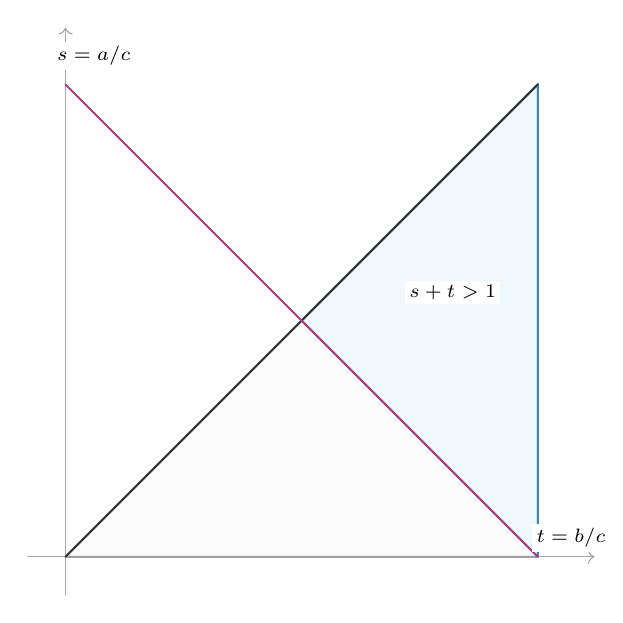
\begin{tikzpicture}[scale=6.000000,line cap=round,line join=round]
\path[use as bounding box] (-0.08000000,-0.08000000) rectangle (1.12000000,1.12000000);
\draw[->,black!35] (-0.08000000,0)--(1.12000000,0);
\draw[->,black!35] (0,-0.08000000)--(0,1.12000000);
\draw[draw=black!38,fill=black!3,line width=.7pt,fill opacity=.55] (0.00000000,0.00000000) -- (1.00000000,0.00000000) -- (1.00000000,1.00000000) -- cycle;
\draw[draw=cyan!65!black,fill=cyan!10,line width=.7pt,fill opacity=.55] (0.50000000,0.50000000) -- (1.00000000,0.00000000) -- (1.00000000,1.00000000) -- cycle;
\draw[draw=black!80,line width=.7pt] (0.00000000,0.00000000) -- (1.00000000,1.00000000);
\draw[draw=magenta!70!black,line width=.7pt] (0.00000000,1.00000000) -- (1.00000000,0.00000000);
\node[font=\scriptsize,fill=white,inner sep=1.5pt] at (1.07000000,0.04000000) {\(t=b/c\)};
\node[font=\scriptsize,fill=white,inner sep=1.5pt] at (0.06000000,1.06000000) {\(s=a/c\)};
\node[font=\scriptsize,fill=white,inner sep=1.5pt] at (0.82000000,0.56000000) {\(s+t>1\)};
\end{tikzpicture}

\end{center}

\subsection*{5. 鋭角領域を円弧で積分する}

最大の辺に対する鋭角条件を単位円の外側として描き、断面の長さを積分します。最後に、三枚を小さい順に並べた全領域の体積で割ります。

\[
\frac{\displaystyle\int_0^1\int_{c/\sqrt2}^{c}\left(b-\sqrt{c^2-b^2}\right)\,db\,dc}{1/6}=1-\frac\pi4
\]

\begin{center}

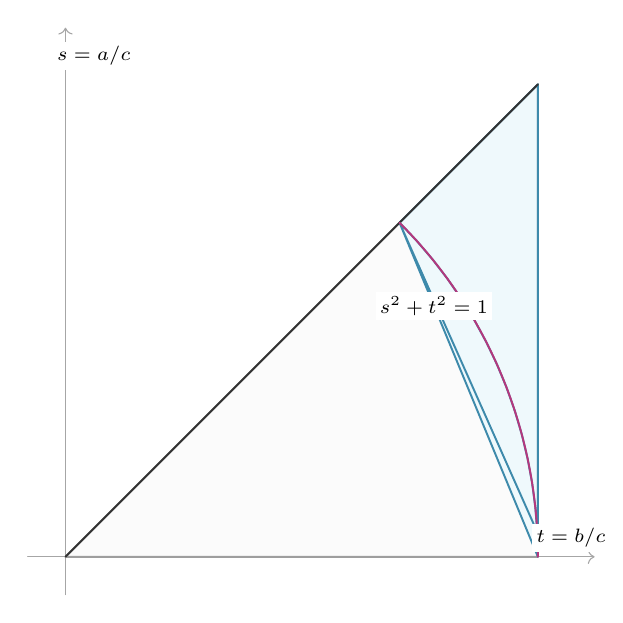
\begin{tikzpicture}[scale=6.000000,line cap=round,line join=round]
\path[use as bounding box] (-0.08000000,-0.08000000) rectangle (1.12000000,1.12000000);
\draw[->,black!35] (-0.08000000,0)--(1.12000000,0);
\draw[->,black!35] (0,-0.08000000)--(0,1.12000000);
\draw[draw=black!38,fill=black!3,line width=.7pt,fill opacity=.55] (0.00000000,0.00000000) -- (1.00000000,0.00000000) -- (1.00000000,1.00000000) -- cycle;
\draw[draw=cyan!65!black,fill=cyan!10,line width=.7pt,fill opacity=.55] (0.70710678,0.70710678) -- (1.00000000,1.00000000) -- (1.00000000,0.00000000) -- (0.70710678,0.70710678) -- (0.74314483,0.66913061) -- (0.77714596,0.62932039) -- (0.80901699,0.58778525) -- (0.83867057,0.54463904) -- (0.86602540,0.50000000) -- (0.89100652,0.45399050) -- (0.91354546,0.40673664) -- (0.93358043,0.35836795) -- (0.95105652,0.30901699) -- (0.96592583,0.25881905) -- (0.97814760,0.20791169) -- (0.98768834,0.15643447) -- (0.99452190,0.10452846) -- (0.99862953,0.05233596) -- cycle;
\draw[draw=black!80,line width=.7pt] (0.00000000,0.00000000) -- (1.00000000,1.00000000);
\draw[draw=magenta!70!black,line width=.7pt] (1.00000000,0.00000000) arc[start angle=0.00000000,end angle=45.00000000,radius=1.00000000];
\node[font=\scriptsize,fill=white,inner sep=1.5pt] at (1.07000000,0.04000000) {\(t=b/c\)};
\node[font=\scriptsize,fill=white,inner sep=1.5pt] at (0.06000000,1.06000000) {\(s=a/c\)};
\node[font=\scriptsize,fill=white,inner sep=1.5pt] at (0.78000000,0.53000000) {\(s^2+t^2=1\)};
\end{tikzpicture}

\end{center}

\section*{講評}
\noindent\textbf{出題意図}\quad 確率・統計・整数の条件を実行可能な関係へ移し、数式を正確に読み取る、計算できる式に直す、整数標本を格子点計数と体積比で解くを一つの証明として組み立てる力を問う。

\noindent\textbf{想定する入試}\quad 新課程の確率・統計を含む記述式入試を想定し、数値だけでなく確率変数の定義、期待値・分散・共分散の導出までを採点対象とする。

\noindent\textbf{独自性}\quad 数値近似や答えの照合で終えず、問題文から答えまで実際に通過した射と証明義務を再生できる。


\section*{証明の経路}
\begin{center}
\begin{tikzpicture}[
  node distance=3.5mm,
  stage/.style={draw,rounded corners=1pt,align=left,text width=118mm,minimum height=7mm,inner xsep=4pt,inner ysep=2pt,font=\small},
  flow/.style={-{Latex[length=2mm]},thick,cyan!55!black},
  edge label/.style={fill=white,inner xsep=3pt,font=\scriptsize\bfseries}
]
\node[stage] (n0) {問題文};
\node[stage,below=of n0] (n1) {読み取った数式};
\draw[flow] (n0) -- node[edge label] {数式を正確に読み取る} (n1);
\node[stage,below=of n1] (n2) {厳密計算用の式};
\draw[flow] (n1) -- node[edge label] {計算できる式に直す} (n2);
\node[stage,below=of n2] (n3) {整数標本の格子点計数と体積比};
\draw[flow] (n2) -- node[edge label] {整数標本を格子点計数と体積比で解く} (n3);
\node[stage,below=of n3] (n4) {検証済み解答};
\draw[flow] (n3) -- node[edge label] {証明書を再生して結論を認証} (n4);
\end{tikzpicture}
\end{center}

\clearpage
\section*{使った射と役割}
\begin{itemize}
\item \textbf{M1: 数式を正確に読み取る}\\
問題文
$\longrightarrow$
読み取った数式\\
文字、演算、等号、積分区間を区別し、元の数式の構造を保つ。
\item \textbf{M2: 計算できる式に直す}\\
読み取った数式
$\longrightarrow$
厳密計算用の式\\
読み取った数式を、分数や根号を保った厳密計算用の式へ移す。
\item \textbf{M3: 整数標本を格子点計数と体積比で解く}\\
厳密計算用の式
$\longrightarrow$
整数標本の格子点計数と体積比\\
相異なる整数を昇順に並べ、有限の場合は格子点を数え、極限では同じ不等式が定める領域の体積へ移す。
\item \textbf{M4: 証明書を再生して結論を認証}\\
整数標本の格子点計数と体積比
$\longrightarrow$
検証済み解答\\
実行記録と証明義務を再生し、元の問題条件に対する結論を確定する。
\end{itemize}




\section*{検証記録}
\begin{itemize}
\item LaTeX数式を構文解析
\item 型付きの実行可能式へ変換
\item 整数標本の格子点計数と体積比 で厳密計算
\item 未評価演算と制約残差を検査
\item 問題文・解答・検証証明書を出力
\end{itemize}
\noindent\textbf{検証方法}\quad 現在の問題文から合成した証明を、厳密な記号計算と図の根拠から再生
\par\noindent{\footnotesize 証明書 SHA-256: \nolinkurl{d95437e60cd77a582c5b864b892c17210515ea08b803f9559e118672e491675a}}

\end{document}
